\documentclass{article}
% =======PACKAGES=======
% FORMATTING
\usepackage[margin=0.625in]{geometry}
\usepackage{parskip, setspace}
\setstretch{1.15}
% TYPESETTING - MATH
\usepackage{amsmath, amsfonts}
\usepackage{amsthm}
\usepackage[ruled, linesnumbered, noend]{algorithm2e}
\NewCommandCopy{\legacyunderscore}{\_}
\renewcommand{\_}{\ifincsname_\else\legacyunderscore\fi}
\usepackage{listings}
\usepackage{xcolor}
\usepackage{algorithm2e}

\lstdefinestyle{mystyle}{
    backgroundcolor=\color{lightgray},   
    commentstyle=\color{darkgray},
    keywordstyle=\color{red},
    numberstyle=\color{black},
    stringstyle=\color{violet},
    basicstyle=\ttfamily\footnotesize,
    breakatwhitespace=false,         
    breaklines=true,                 
    captionpos=b,                    
    keepspaces=true,                 
    numbers=left,                    
    numbersep=5pt,                  
    showspaces=false,                
    showstringspaces=false,
    showtabs=false,                  
    tabsize=2
}
\lstset{style=mystyle}
% RICH
\usepackage{graphicx, caption}
\usepackage{hyperref}
% BIBLIOGRAPHY
\usepackage[
backend=biber,
sorting=ynt
]{biblatex}
\addbibresource{bib.bib}

\newcommand{\integer}{\textbf{int} }

% =======TITLE=======
\title{\vspace*{-0.625in}CS 529: Advanced Data Structures \& Algorithms \\ Assignment 6: Genetic Algorithms}
\author{Nathan Chapman, Hunter Lawrence, Andrew Struthers}
\date{\today}

\begin{document}

\maketitle

\section*{Eye Color}

    Consider the eye color of a human being as determined by the bey2 gene.  Recall that the allele for brown eyes is dominant.  For each of the following parent allele combinations, determine the eye color of the individual.

    \underline{\textbf{Solution}}

    Example 10.1 defines the BLUE gene as recessive because ``if an individual receives one BLUE allele and one BROWN ellele, that individual will have brown eyes''.  Therefore the possibilities can be exaushtively enumerated as in table \ref{tbl:eye_color}.

    \begin{table}[h]
        \centering
        \begin{tabular}{|c|c|c|}
            \hline
            Father & Mother & Child \\
            \hline
            BLUE   & BLUE   & BLUE  \\
            \hline
            BLUE   & BROWN  & BROWN \\
            \hline            
            BROWN  & BLUE   & BROWN \\
            \hline
            BROWN  & BROWN  & BROWN \\
            \hline
        \end{tabular}
        \caption{Eye color of child given eye color of parents being either blue or brown}
        \label{tbl:eye_color}
    \end{table}

    Because there are only two possibilities, they can be exactly represented as boolean values as BLUE $\equiv false$ and BROWN $\equiv true$; alternatively, each value is the truth value of the statement ``This parent has brown eyes''.  Furthermore, due to the dominant nature of the BROWN gene, the child's eye color can be effectively determined by an OR operation on the parents eye colors.  With this representation in mind, we can exactly represent the data and relationships dentoed in table \ref{tbl:eye_color} by those in the truth table \ref{tbl:eye_color_truth}.

    \begin{table}[h]
        \centering
        \begin{tabular}{|c|c|c|}
            \hline
            Father & Mother & Child \\
            \hline
            False  & False  & False \\
            \hline
            False  & True   & True \\
            \hline            
            True   & False  & True \\
            \hline
            True   & True   & True \\
            \hline
        \end{tabular}
        \caption{Truth table representation of table \ref{tbl:eye_color}}
        \label{tbl:eye_color_truth}
    \end{table}

    Likewise, these data can also be represented as bits allowing for bitwise-OR operations.
\newpage
\section*{The Traveling Sales Problem}
Assume the weights in both directions on an edge are the same. Find the shortest tour. Analyze how the genetic approach is justified for this task.
\begin{figure}[!h]
    \centering
    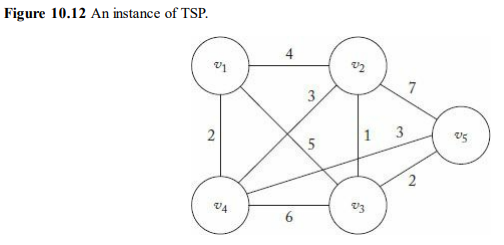
\includegraphics[width=0.5\textwidth,keepaspectratio]{tsp.png}
    \label{fig:space_partition}
    \caption{5 vertex weighted graph representing an instance of the Travelling Salesperson Problem}
\end{figure}
$ $\\
\underline{\textbf{Solution}}\\
There are many ways we can approach this problem. The intuitive way to start thinking about this problem is simply start looking for edges that have lower weights. For example, we can see that the edge between $v_2$ and $v_3$ has a weight of $1$, whereas no other path starting from a vertex and ending at either $v_2$ or $v_3$ is that inexpensive. This gives us the intuition that the edge from $v_2$ to $v_3$ should at least be considered when looking for the full tour. Once we have identified this feature of the graph, an intuitive guess-and-check method of finding all tours that contain the edge $\{v_2, v_3\}$. To do this, we can employ a greedy or nearest neighbor style approach. If we arbitrarily say we want to start with the tour $\{v_3, v_2\}$, the greedy approach would be to then travel from $v_2$ to $v_4$, then from $v_4$ to $v_1$. However, once we have got to $v_1$ following this path, we can no longer continue. $v_1$ only has an edge to $v_2$, $v_3$, and $v_4$. We have not visited $v_5$, and as such we do not have a full tour. This tells us that using a greedy approach starting at $v_3$ does not yield a valid tour. Since we have a really strong intuition telling us that the edge $\{v_2, v_3\}$ should be included in our tour, let's instead start at $v_2$. The greedy approach would tell us to go to $v_3$, which is the edge we wanted. Then, we would go to $v_5$, then from $v_5$ to $v_4$, then from $v_4$ to $v_1$, then we only have to visit $v_2$ again to end our tour. This is a valid tour, and has a cost of $1 + 2 + 3 + 2 + 4 = 12$. Likewise, the greedy approach would have found the same tour starting from $v_4$ and $v_1$. The $v_1$ route is tricky, because there's a tie at the edges $\{v_4, v_2\}$ and $\{v_4, v_5\}$. In this case, the greedy algorithm would have to explore both paths. \\\\
Another approach could be taken. If we consider all the edges in this graph, we can sort them from shortest to longest. In order of least to greatest edge cost, we have $\left\{\{v_2, v_3\}, \{v_1, v_4\}, \{v_3, v_5\}, \{v_2, v_4\}, \{v_4, v_5\}, \{v_1, v_2\}, \{v_1, v_3\}, \{v_3, v_4\}, \{v_2, v_5\}\right\}$. We can now do a simple algorithm, where we remove the edge with the highest cost if and only if removing it doesn't result no possible complete tours of the graph. For example, we can remove edge $\{v_3, v_4\}$, and there is still at least 1 valid tour that reaches each node exactly once and returns to the starting node. So, first we remove edge $\{v_2, v_5\}$, as it is the edge with the highest cost and doing so doesn't result in a graph with 0 valid tours. The next highest edge is $\{v_3, v_4\}$, so we remove that one as well. The new highest cost edge is $\{v_1, v_3\}$, and removing that doesn't make a graph with no possible tours. The next highest cost edge is $\{v_1, v_2\}$, which if we deleted it, would in fact make a graph that has no possible tours. If we remove that edge, there is only one edge travelling to $v_1$, which would break our rules of only visiting each vertex once, and ending at the starting vertex. Therefore, we can't remove $\{v_1, v_2\}$. The next highest edge is $\{v_4, v_5\}$, which just like before, if we removed that edge there would be only one route into $v_5$, so we can't remove it. Then after that, we have edge $\{v_2, v_4\}$. If we removed that edge, we would still have at least one valid tour. At this point, we have the edges $\left\{\{v_2, v_3\}, \{v_1, v_4\}, \{v_3, v_5\}, \{v_4, v_5\}, \{v_1, v_2\} \right\}$. A tour through 5 vertices requires exactly 5 edges, and we are now left with a set of 5 edges. It is clear to see that if we removed any one of these edges, we would no longer have a valid tour through the graph. We can count up the weights of all of these edges, and we will have $1 + 2 + 2 + 3 + 4 = 12$. This algorithm borrows ideas from the Max-Flow, Min-Cut theorem in graph theory, which states that the maximum ``flow" passing from some source vertex to some sink vertex (in this case it can be the same vertex) is equal to the total weight of the edges in a minimum cut. The minimum cut is defined as the smallest sum of all weights of edges, which, if removed, would disconnect the source from the sink. In our case, we have done exactly that. We have found the smallest sum of all weights of edges, where if we were to remove any of the edges, we would disconnect the starting vertex from itself. Therefore we have shown that both the greedy approach starting at vertices $v_1$, $v_2$, and $v_4$ as well as the simple algorithm derived from the ideas inside the Max-Flow, Min-Cut theorem are both capable of generating the shortest tour. \\\\
This task is a task suitable for a genetic approach because genetic algorithms are well-suited for exploring large solution spaces efficiently. In the case of finding the shortest tour, there could be a vast number of possible permutations of routes to consider. In this specific example, there are only a few permutations that create a possible tour, but in general there can be many permutations. Genetic algorithms can systematically explore these spaces by maintaining a population of candidate solutions and iteratively improving them through genetic operations such as crossover and mutation. In crossover, only children solutions that improve upon their parents are considered and passed to future generations, so from an initial population of random solutions we can iteratively work towards a better solution. Because solutions to the TSP can be encoded as a set of vertices, we can perform the standard selection, crossover, and mutation to create genome sequences where each allel is a unique identifier of a vertex. Using the iterative approach of systematically exploring and improving upon solutions, genetic algorithms can find a good balance of exploration and exploitation to solve the TSP effectively.  

\section*{Genetic Algorithms and Financial Trading}
A major search area for adaptive applications is in financial sector. The hunt for an application that can use historical trade data to predict the outcome of future markets is a continuing task. One approach to solve this is the use of genetic programming trained on historical data to search for an optimal decision process. One realization of this approach involved taking historical data of financial markets (particularly the S\&P500 index from 1983 to 2004). The terminal symbols for this included \textbf{$SP500$} performance over the past 200 days:\\
Where $SP500_{avg}$ is the average value for the past 200 days, $SP500_{today}$ is the value of the current day, and $SP_\sigma$ is the standard deviation of the value of the past 200 days:

\begin{equation}
    \begin{aligned}
     SP500 = \frac{SP500_{today} - SP500_{avg}}{SP500_\sigma}
     \end{aligned}
\end{equation}

The Moving Average Convergence/Divergence (\textbf{$MACD$}), which measures how the k-day Exponential Moving Average ($EMA$) (the weighted average of a security of the past k-days) is changing:
Where $x$ is the security being evaluated:

\begin{equation}
    \begin{aligned}
     MACD(x) = 12\text{-}day EMA(x) - 26\text{-}day EMA(x)
     \end{aligned}
\end{equation}

The \textbf{$MACD9$} is the 9-day EMA for the $S\&P500$
The McClennan Oscilator ($MCCL$) is a consideration on whether a market is overbought (when $MCCL > 100$) or oversold (When $MCCL < -100$) and can be modeled by the following:\\
Where $diff$ is the difference of the  umber of advancing and declining securities:

\begin{equation}
    \begin{aligned}
    MCCL = 19\text{-}day EMA(diff) - 39\text{-}day EMA(diff).
    \end{aligned}
\end{equation}

Indicators with the postfix ``-lag" are the values of those indicators on the previous day. Real constants in range $[-1, 1]$ are also adjusted from generation to generation.

An example of this algorithm can be seen in the figure below. In this example, $IFGT$ compares its first two child values, and if the first is greater than the second, then the third child node is executed and returned, otherwise, the second is returned. $IF$ conditionals will return the second child node if the first node is greater than zero, otherwise, the third will return.
\begin{figure}[!h]
    \centering
    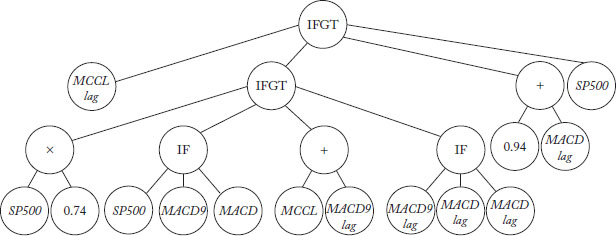
\includegraphics[width=0.5\textwidth,keepaspectratio]{gen_alg_tree.jpg}
    \label{fig:space_partition}
    \caption{Generated program tree for determining to buy, hold, or sell on the S\&P 500 index from 1983 to 2004}
\end{figure}
\newpage
This example can be be modeled in the following algorithm:

\begin{algorithm}[!h]
    \DontPrintSemicolon
    \caption{Execution order of the tree in generated program tree above}
    \label{alg:sp500}
    \KwResult{A metric to determine if the user should buy, hold, or sell}

    $IF\_1$\;
    \If {$SP500 > 0$}
    {
        $IF\_1 \gets MACD9$\;
    }
    \Else
    {
        $IF\_1 \gets MACD$\;
    }
    $IFGT\_1$\;
    \If{$SP500*0.74 > IF\_1$}
    {
        $IFGT\_1 \gets MCCL + MACD9_{lag}$\;
    }
    \Else
    {
        \If{$MACD9_{lag} > 0$}
        {
            $IFGT\_1 \gets MACD_{lag}$\;
        }
        \Else
        {
            $IFGT\_1 \gets MACD_{lag}$\;
        }
    }
    \If{$MCCL_{lag} > IFGT\_1$}
    {
        \Return{$0.94 + MACD_{lag}$}\;
    }
    \Else
    {
        \Return{$SP500$}\;
    }
\end{algorithm}


Applications for these kinds of trees extend beyond financial prediction, and into machine learning. As solutions to problems are generated and evaluated against existing data sets, accurate predictions can be created based on new data. This has application for the creation of predictive algorithms that can be used to evaluate not only financial risk, but also predict medical conditions based on some set of data from a patient, consumer behaviors, weather patterns, etc.  

\end{document}